\chapter{Scaling bitcoin}

There is no secret that the bitcoin blockchain will not be able to scale on its own. When Nakamoto first published the whitepaper on the cryptographic mailing list his first response was in fact that such a solution won't scale very well\cite{donald:scale}. 

Andreas Antonopoulos has drawn similarities between the scaling of bitcoin with the scaling of the internet:

\begin{displayquote}
	"Bitcoin is failing to scale. If we’re really lucky, bitcoin will continue to fail to scale gracefully for 25 years, just like the internet."\cite{antonopoulos:the:internet:of:money}
\end{displayquote}

His quote in many ways are spot on as Usenet used a \textit{Store-and-forward} method for content to reach every server in the network. \textit{Store-and-forward} does not scale very well and is somewhat similar to the base Bitcoin protocol. The internet moved away from \textit{Store-and-forward} to more direct routing and Bitcoin is too, allowing transactions to happen off-chain.

In this chapter the various scaling alternatives will be discussed.

\section{Block Size limit}

In 2010 Nakamoto reduced the block size limit from 32 to 1 Megabyte as part of two commits. The first commit introduces the new \texttt{BLOCK\_SIZE\_LIMIT} constant\cite{nakamoto:commit:1} and the other commit enforcing the blocks to be under the limit\cite{nakamoto:commit:2}. Nakamoto did not give any explanation as to the reason of this limit. As there was only a few transactions per block at this time a limit reduced the worst case scenario for a DoS attacker filling up the blocks with dummy transactions. 

Increasing the amount of transactions would also increase the imposing cost for the ecosystem by forms of bandwidth, processing, storage and the speed by which blocks propagate through the network. By imposing a block limit the cost of operating a node would be kept low allowing more peers to be able to participate in the network. 

% would come at an increased cost for the ecosystem (bandwidth, processing, and storage for relay nodes, as well as an impact on propagation speed of blocks on the network

% TODO: Math example, compare visa 

\section{Increasing block size limit}

There has been many proposals to increase the block size. Including a handful of BIPs:

\begin{itemize}
	
	\item \textbf{BIP 100} allows the miner to vote on the block limit by encoding a proposed value in the coinbase unlocking script. A 75\% supermajority may increase the block size limit every 2016 blocks. Each period change is limited to only increase by 5\% from the previous period.\cite{bip:0100:dynamic:block:size}
	
	\item \textbf{BIP 101} proposes an immediate increase to 8 megabyte blocks and continue to double every second year. In the two year periods the size would increase at a linear pace based on the block timestamp.\cite{bip:0101:increase:block:size}
	
	\item \textbf{BIP 102} is a simple one time increase to 2 megabytes. The BIP would be triggered if 95\% of the latest blocks signaled support for the upgrade.\cite{bip:0102:increase:2mb}
	
	\item \textbf{BIP 103} aims to increase the block size in accordance with the technology. In practice however it increases the block size with 4.4\% every ~97 day, 17.7\% annually. \cite{bip:0103:increase:with:technology}
\end{itemize}

Most of these BIPs are implemented as a hard forks. Older nodes would regard the bigger blocks as being over the limit and thus invalid.
If poorly executed, without a great majority upgrading the software in time, the network would be forked into two networks with diverging transaction histories. 

% need better name for community worker
\subsection{Contentious Hard Forks}

No proposal to increase the block size has yet received enough support to be activated. This has caused some controversy among community members and multiple have attempted to increase the limit by force. 

One of the earliest attempts to increase the block size was when node Bitcoin XT implemented BIP 101 mentioned above. It failed to reach the miner consensus it required to activate. The BIP 101 was then removed and replaced by a 2 megabyte block limit which forked bitcoin into a new network known as bitcoin classic. Mike Hearn, co-creator of Bitcoin XT along with Gavin Andersen, has made his intention clear arguing that the block size must increase for bitcoin to reach any adoption beyond a fringe niche\cite{hearn:classic}. 

\begin{figure}[!htb]
	\hspace*{-0.7cm} 
	\centering
	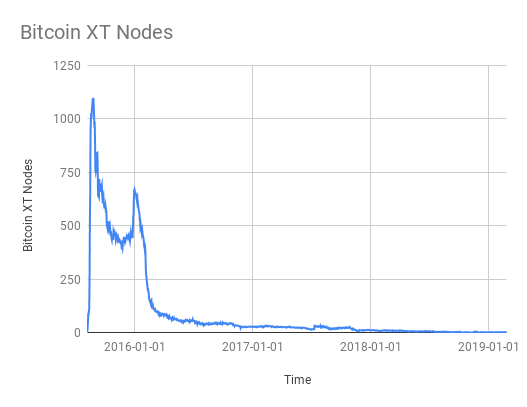
\includegraphics[width=8cm]{external/Bitcoin_XT_Nodes.png}
	\caption{\textit{Historic Bitcoin XT node count. As of 2019-02-25 only 3 nodes are still active. Data retrieved from coin.dance\cite{coin:dance}.}}
	\label{fig:xt_nodes}
	\hspace*{2mm} 	
\end{figure}

As figure \ref{fig:xt_nodes} attests, bitcoin XT and classic failed to receive support and is now dead. 

\subsection{The bitcoin cash saga}

\begin{itemize}
	\item SegWit2x
\end{itemize} 


( THIS SECTION IS OBVOUSLY NOT DONE) 

\section{Removing decentralization}

\section{Side channel}

\section{Off-chain scaling}

\section{Rational for a small blocks}
